\documentclass[UTF8,zihao=-4,scheme=chinese,fontset=none]{ctexart}

\usepackage[a4paper,top=2.5cm,bottom=2.5cm,left=2.8cm,right=2.8cm,headheight=15pt]{geometry}
\usepackage{fontspec}
\usepackage{xeCJK}
\usepackage{setspace}
\usepackage{indentfirst}
\usepackage{fancyhdr}
\usepackage{booktabs}
\usepackage{tabularx}
\usepackage{array}
\usepackage{longtable}
\usepackage{graphicx}
\usepackage{float}
\usepackage{caption}
\usepackage{tikz}
\usetikzlibrary{arrows.meta,positioning,shapes.geometric}
\usepackage{listings}
\usepackage{xcolor}
\usepackage{enumitem}
\usepackage{amsmath}
\usepackage{url}
\usepackage[hidelinks,unicode]{hyperref}

\IfFileExists{fonts/times.ttf}{
  \setmainfont[
    Path=fonts/,
    BoldFont=timesbd.ttf,
    ItalicFont=timesi.ttf,
    BoldItalicFont=timesbi.ttf
  ]{times.ttf}
}{\setmainfont{TeX Gyre Termes}}
\IfFileExists{fonts/simsun.ttc}{
  \setCJKmainfont[Path=fonts/,AutoFakeBold=2.5]{simsun.ttc}
  \setCJKmonofont[Path=fonts/]{simsun.ttc}
}{
  \setCJKmainfont[AutoFakeBold=2.5]{FandolSong-Regular}
  \setCJKmonofont{FandolFang-Regular}
}
\IfFileExists{fonts/simhei.ttf}{
  \setCJKsansfont[Path=fonts/]{simhei.ttf}
  \setCJKfamilyfont{hei}[Path=fonts/]{simhei.ttf}
}{
  \setCJKsansfont{FandolHei-Regular}
  \setCJKfamilyfont{hei}{FandolHei-Regular}
}
\newcommand{\heiti}{\CJKfamily{hei}}

\setlength{\parindent}{2em}
\setlength{\parskip}{0pt}
\linespread{1.35}
\setlength{\emergencystretch}{2em}
\renewcommand{\arraystretch}{1.22}
\setlist{nosep,leftmargin=2em}
\setcounter{tocdepth}{2}
\graphicspath{{figures/}}

\ctexset{
  section={
    format=\heiti\zihao{3},
    name={第,章},
    number=\chinese{section},
    beforeskip=0.8em,
    afterskip=0.7em
  },
  subsection={
    format=\heiti\zihao{4},
    beforeskip=0.7em,
    afterskip=0.4em
  },
  subsubsection={
    format=\heiti\zihao{-4},
    beforeskip=0.5em,
    afterskip=0.3em
  }
}

\captionsetup{font=small,labelsep=quad}
\DeclareCaptionFont{heiti}{\heiti}
\captionsetup{labelfont=heiti}
\renewcommand{\contentsname}{目\quad 录}
\renewcommand{\refname}{参考文献}

\pagestyle{fancy}
\fancyhf{}
\fancyhead[C]{\zihao{5}实验一：目标检测与识别}
\fancyfoot[C]{\thepage}
\renewcommand{\headrulewidth}{0.4pt}
\renewcommand{\footrulewidth}{0pt}

\definecolor{codegray}{gray}{0.95}
\lstset{
  basicstyle=\ttfamily\zihao{5},
  backgroundcolor=\color{codegray},
  frame=single,
  rulecolor=\color{black},
  breaklines=true,
  columns=fullflexible,
  keepspaces=true,
  showstringspaces=false,
  numbers=left,
  numberstyle=\tiny,
  xleftmargin=2em,
  framexleftmargin=1.5em
}

\newcolumntype{Y}{>{\raggedright\arraybackslash}X}
\newcommand{\githuburl}{\url{https://github.com/xhr-CHN/jetson-ros2-object-detection}}
\newcommand{\passmark}{\heiti 通过}

\begin{document}

\begin{titlepage}
  \thispagestyle{empty}
  \begin{center}
    \vspace*{2.2cm}
    {\heiti\zihao{1} 实验一：目标检测与识别\par}
    \vspace{0.8cm}
    {\heiti\zihao{2} 基于 YOLO26n、Jetson 与 ROS 2 的\par}
    \vspace{0.3cm}
    {\heiti\zihao{2} 铅笔和网球检测系统\par}

    \vspace{2.4cm}
    \renewcommand{\arraystretch}{1.8}
    \begin{tabular}{>{\heiti}p{3.2cm}p{8.2cm}}
      课程名称： & 机器人集成实验 \\
      实验名称： & 目标检测与识别 \\
      姓\qquad 名： & \hrulefill \\
      学\qquad 号： & \hrulefill \\
      班\qquad 级： & \hrulefill \\
      实验日期： & 2026年8月24日--2026年8月30日 \\
      GitHub： & \href{https://github.com/xhr-CHN/jetson-ros2-object-detection}{xhr-CHN/jetson-ros2-object-detection} \\
    \end{tabular}

    \vfill
    {\heiti\zihao{3} 2026年8月30日\par}
  \end{center}
\end{titlepage}

\pagenumbering{Roman}
\setcounter{page}{1}

\section*{摘\quad 要}
\addcontentsline{toc}{section}{摘要}

本实验面向桌面物体目标检测任务，选取铅笔和网球两类物体，完成数据集整理、YOLO格式标注统一、YOLO26n模型训练、独立测试集评估、Jetson Orin部署以及ROS 2检测结果发布。项目合并Mendeley Data、Kaggle与Roboflow Universe的四个公开数据来源，将五种铅笔子类别统一为\texttt{pencil}，将网球统一为\texttt{tennis\_ball}。最终数据集包含895张图片和1048个标注目标，其中训练集605张、验证集171张、测试集119张。测试集未参与训练和最佳权重选择。

模型在NVIDIA GeForce RTX 4060 Laptop GPU上完成100轮正式增强训练，最佳权重出现在第87轮。验证集Precision为0.96338、Recall为0.97329、mAP@0.5为0.98185、mAP@0.5:0.95为0.88025。独立测试集总体Precision为0.98877、Recall为0.90186、mAP@0.5为0.97148、mAP@0.5:0.95为0.87761。模型导出为PyTorch、ONNX和TensorRT Engine三种格式，并在Jetson Orin上以ROS 2 Humble节点运行。摄像头检测图像话题平均速率为13.795 FPS，节点发布检测FPS平均为16.657 FPS，均高于5 FPS验收线。

最终板端验收采用第二次测试记录，只从留出测试集固定抽取铅笔20张和网球20张。40项中正确39项，总正确率97.5\%；铅笔正确率95.0\%，网球正确率100.0\%。唯一错误为红色铅笔漏检，错误样本和全部40张结果图均保留。实验代码、数据、模型、视频、运行说明与分阶段提交记录公开保存于GitHub。本实验结果满足课程提出的两类物体、正确率不低于80\%、Jetson实时速度不低于5 FPS、ROS 2发布及保留典型错误案例等要求。

\noindent\textbf{关键词：}目标检测；YOLO26n；Jetson Orin；TensorRT；ROS 2；铅笔；网球

\clearpage
\begingroup
  \zihao{5}\linespread{1.0}\selectfont
  \tableofcontents
\endgroup
\clearpage

\pagenumbering{arabic}
\setcounter{page}{1}

\section{实验任务与总体完成情况}

\subsection{实验任务}

课程要求选择不少于两类桌面物体，自行完成数据采集或公开数据整理与标注，训练目标检测模型，在Jetson上实时显示目标类别、检测框与置信度，并通过ROS 2发布识别结果。验收还要求测试不少于20个物体、正确识别率不低于80\%、Jetson实时检测速度不低于5 FPS，以及保存测试结果和典型错误案例。提交材料包括数据集、模型、程序、结果视频、运行说明和LaTeX实验报告。

本项目将任务具体化为\texttt{pencil}与\texttt{tennis\_ball}两类桌面目标。之所以选择这两类物体，一是二者形状差异明显，适合验证检测器的多尺度能力；二是铅笔细长、网球近圆，两者在尺度、长宽比和背景干扰方面具有互补性；三是实物易获取，便于在USB摄像头和Jetson现场展示。

\subsection{验收指标对照}

\begin{table}[H]
  \centering
  \caption{课程要求与真实完成结果对照}
  \begin{tabularx}{\textwidth}{Y Y Y c}
    \toprule
    要求 & 验证方法 & 实际结果 & 结论 \\
    \midrule
    不少于2类物体 & 检查类别配置与演示画面 & 铅笔、网球2类 & \passmark \\
    测试不少于20个物体 & Jetson第二次固定验收 & 共40项，每类20项 & \passmark \\
    正确率不低于80\% & 统计40项预测结果 & 39/40，97.5\% & \passmark \\
    Jetson速度不低于5 FPS & 话题速率和节点FPS采样 & 13.795/16.657 FPS & \passmark \\
    显示框、类别、置信度 & 最终视频抽帧与程序检查 & 两类均实时显示 & \passmark \\
    ROS 2发布结果 & 节点与话题记录 & 三个检测话题正常 & \passmark \\
    保存测试与错误案例 & 验收目录完整性检查 & 40张结果图、1个错误案例 & \passmark \\
    \bottomrule
  \end{tabularx}
\end{table}

需要说明的是，97.5\%是固定40项样本的分类式验收正确率，并不等同于目标检测mAP；离线TensorRT速度也不等同于摄像头采集、推理、绘制和ROS 2发布的端到端吞吐量。本报告对这些口径分别陈述，避免将不同指标混用。

\section{系统方案与关键技术}

\subsection{总体流程}

系统按“数据--训练--评估--导出--部署--发布--验收”的顺序实现。Windows计算机负责数据整理、100轮训练和独立测试；Jetson负责生成与本机环境匹配的TensorRT Engine、运行USB摄像头实时检测和ROS 2节点，并保存最终验收证据。完整流程如图\ref{fig:pipeline}所示。

\begin{figure}[H]
  \centering
  \begin{tikzpicture}[
    node distance=5mm,
    box/.style={draw=black,rounded corners=1pt,minimum height=9mm,text width=2.2cm,align=center,font=\small},
    arrow/.style={-Latex,thick}
  ]
    \node[box] (data) {公开数据\\清洗与标注};
    \node[box,right=of data] (train) {YOLO26n\\100轮训练};
    \node[box,right=of train] (test) {独立测试\\指标与图表};
    \node[box,right=of test] (export) {PT/ONNX\\TensorRT};
    \node[box,below=8mm of export] (jetson) {Jetson摄像头\\实时推理};
    \node[box,left=of jetson] (ros) {ROS 2\\三个话题};
    \node[box,left=of ros] (accept) {40项验收\\正确率统计};
    \draw[arrow] (data) -- (train);
    \draw[arrow] (train) -- (test);
    \draw[arrow] (test) -- (export);
    \draw[arrow] (export) -- (jetson);
    \draw[arrow] (jetson) -- (ros);
    \draw[arrow] (ros) -- (accept);
  \end{tikzpicture}
  \caption{系统总体技术流程}
  \label{fig:pipeline}
\end{figure}

\subsection{YOLO26n模型选择}

YOLO系列将类别预测与边界框回归统一在单阶段检测框架中，适合实时应用。YOLO26采用端到端检测设计，默认的一对一检测头可直接输出预测结果，同时简化部署路径；YOLO26n是该系列最小尺度模型，640像素输入下具有较低计算量，适合资源受限的边缘平台\cite{yolo26paper,yolo26docs}。本实验更关注“准确率达到课程阈值并在Jetson稳定实时运行”，因此选择nano尺度，而不是追求更大的模型容量。

边界框标注采用YOLO归一化格式。设图片宽高为$W,H$，目标框左上角为$(x_1,y_1)$、右下角为$(x_2,y_2)$，则标注为
\begin{equation}
  x_c=\frac{x_1+x_2}{2W},\quad
  y_c=\frac{y_1+y_2}{2H},\quad
  w=\frac{x_2-x_1}{W},\quad
  h=\frac{y_2-y_1}{H}.
\end{equation}
每行由类别编号和$(x_c,y_c,w,h)$组成，所有坐标均限制在$[0,1]$范围。

\subsection{评价指标}

Precision、Recall和F1定义为
\begin{equation}
  P=\frac{TP}{TP+FP},\qquad
  R=\frac{TP}{TP+FN},\qquad
  F_1=\frac{2PR}{P+R}.
\end{equation}
mAP@0.5表示交并比阈值为0.5时各类别平均精度的均值；mAP@0.5:0.95是在0.50至0.95多个阈值上的平均结果，更严格地反映定位质量。课程正确识别率则按固定验收样本中“最高置信度预测类别与期望类别一致”计分，空检测记为错误。

\section{数据集构建与标注整理}

\subsection{数据来源与许可}

数据来源、访问日期、原始类别、许可证与处理规则均记录在\path{dataset/SOURCES.md}，避免只保留图片而丢失来源信息。表\ref{tab:sources}列出四个来源。Mendeley网球数据集为CC BY 4.0\cite{mendeley}；Roboflow Pencil v2为CC BY 4.0，Tennis ball v1元数据标记为Public Domain\cite{roboflowpencil,roboflowtennis}。Kaggle Pencil Dataset的公开元数据未提供明确再分发许可证\cite{kagglepencil}，因此本项目仅按课程实验用途记录，后续公开再利用时仍需确认授权。

\begin{table}[H]
  \centering
  \caption{数据来源与处理}
  \label{tab:sources}
  \begin{tabularx}{\textwidth}{Y c c Y}
    \toprule
    来源 & 原始图片 & 许可证 & 本项目处理 \\
    \midrule
    Mendeley Object Detection--Tennis Ball v2 & 150 & CC BY 4.0 & 删除1张完全重复图片，类别映射为网球 \\
    Kaggle Pencil Dataset & 300 & 未明确 & JSON框转YOLO格式，铅笔类别合并 \\
    Roboflow Pencil v2 & 94 & CC BY 4.0 & 五个铅笔子类合并为\texttt{pencil} \\
    Roboflow Tennis ball v1 & 352 & Public Domain & 类别映射为\texttt{tennis\_ball} \\
    \bottomrule
  \end{tabularx}
\end{table}

\subsection{清洗、类别映射与划分}

整理脚本先检查图片能否解码，再检查图片与标签是否成对存在；随后通过文件内容和解码后像素SHA-256进行全局去重。Kaggle JSON中的COCO风格框$[x,y,w,h]$被转换为归一化YOLO格式。所有铅笔外观和颜色均合并为类别0，所有网球合并为类别1。补充数据使用前缀重命名，防止不同来源的同名文件互相覆盖。

\begin{lstlisting}[language={},caption={最终数据配置文件的核心内容}]
path: .
train: images/train
val: images/val
test: images/test
names:
  0: pencil
  1: tennis_ball
\end{lstlisting}

最终统计见表\ref{tab:dataset}。训练集和验证集用于优化与最佳权重选择；119张测试图片在正式模型确定前不参与训练或最佳轮次选择，以保证独立评估。

\begin{table}[H]
  \centering
  \caption{最终YOLO数据集统计}
  \label{tab:dataset}
  \begin{tabular}{lrrr}
    \toprule
    划分 & 图片数 & 铅笔目标数 & 网球目标数 \\
    \midrule
    train & 605 & 317 & 387 \\
    val & 171 & 100 & 94 \\
    test & 119 & 80 & 70 \\
    \midrule
    合计 & 895 & 497 & 551 \\
    \bottomrule
  \end{tabular}
\end{table}

训练目标数量为铅笔317个、网球387个，差距较小；测试集包含60张铅笔图片和59张网球图片。两类源数据的背景风格仍存在差异，这会影响模型对跨域场景的泛化，也是后续可继续补充真实桌面混合场景的原因。

\section{模型训练与验证}

\subsection{训练环境与参数}

正式增强训练只兼容本地Windows环境，由\path{src/train_yolo26n_windows.py}启动。脚本先验证CUDA是否可用，不在GPU失效时静默退回CPU。训练使用NVIDIA GeForce RTX 4060 Laptop GPU，输入尺寸640，批量大小8，总计100轮。完整参数保存在\path{results/training/yolo26n_augmented/args.yaml}，逐轮指标保存在\path{results/training/yolo26n_augmented/results.csv}。

\begin{table}[H]
  \centering
  \caption{正式训练配置}
  \begin{tabular}{ll}
    \toprule
    项目 & 配置 \\
    \midrule
    模型 & YOLO26n预训练权重 \\
    任务 & 两类目标检测 \\
    输入尺寸 & $640\times640$ \\
    Epochs & 100 \\
    Batch size & 8 \\
    设备 & NVIDIA GeForce RTX 4060 Laptop GPU \\
    数据配置 & \path{dataset/data-windows.yaml} \\
    输出目录 & \path{runs/pencil_tennis_yolo26n_augmented} \\
    \bottomrule
  \end{tabular}
\end{table}

\subsection{训练过程}

图\ref{fig:training}为完整100轮训练记录的原始彩色曲线图。训练损失整体下降，验证指标在后期趋于稳定。最佳权重出现在第87轮，而不是人为中断得到的临时权重；本项目最终模型来自完整跑完100轮的正式增强训练。

\begin{figure}[H]
  \centering
  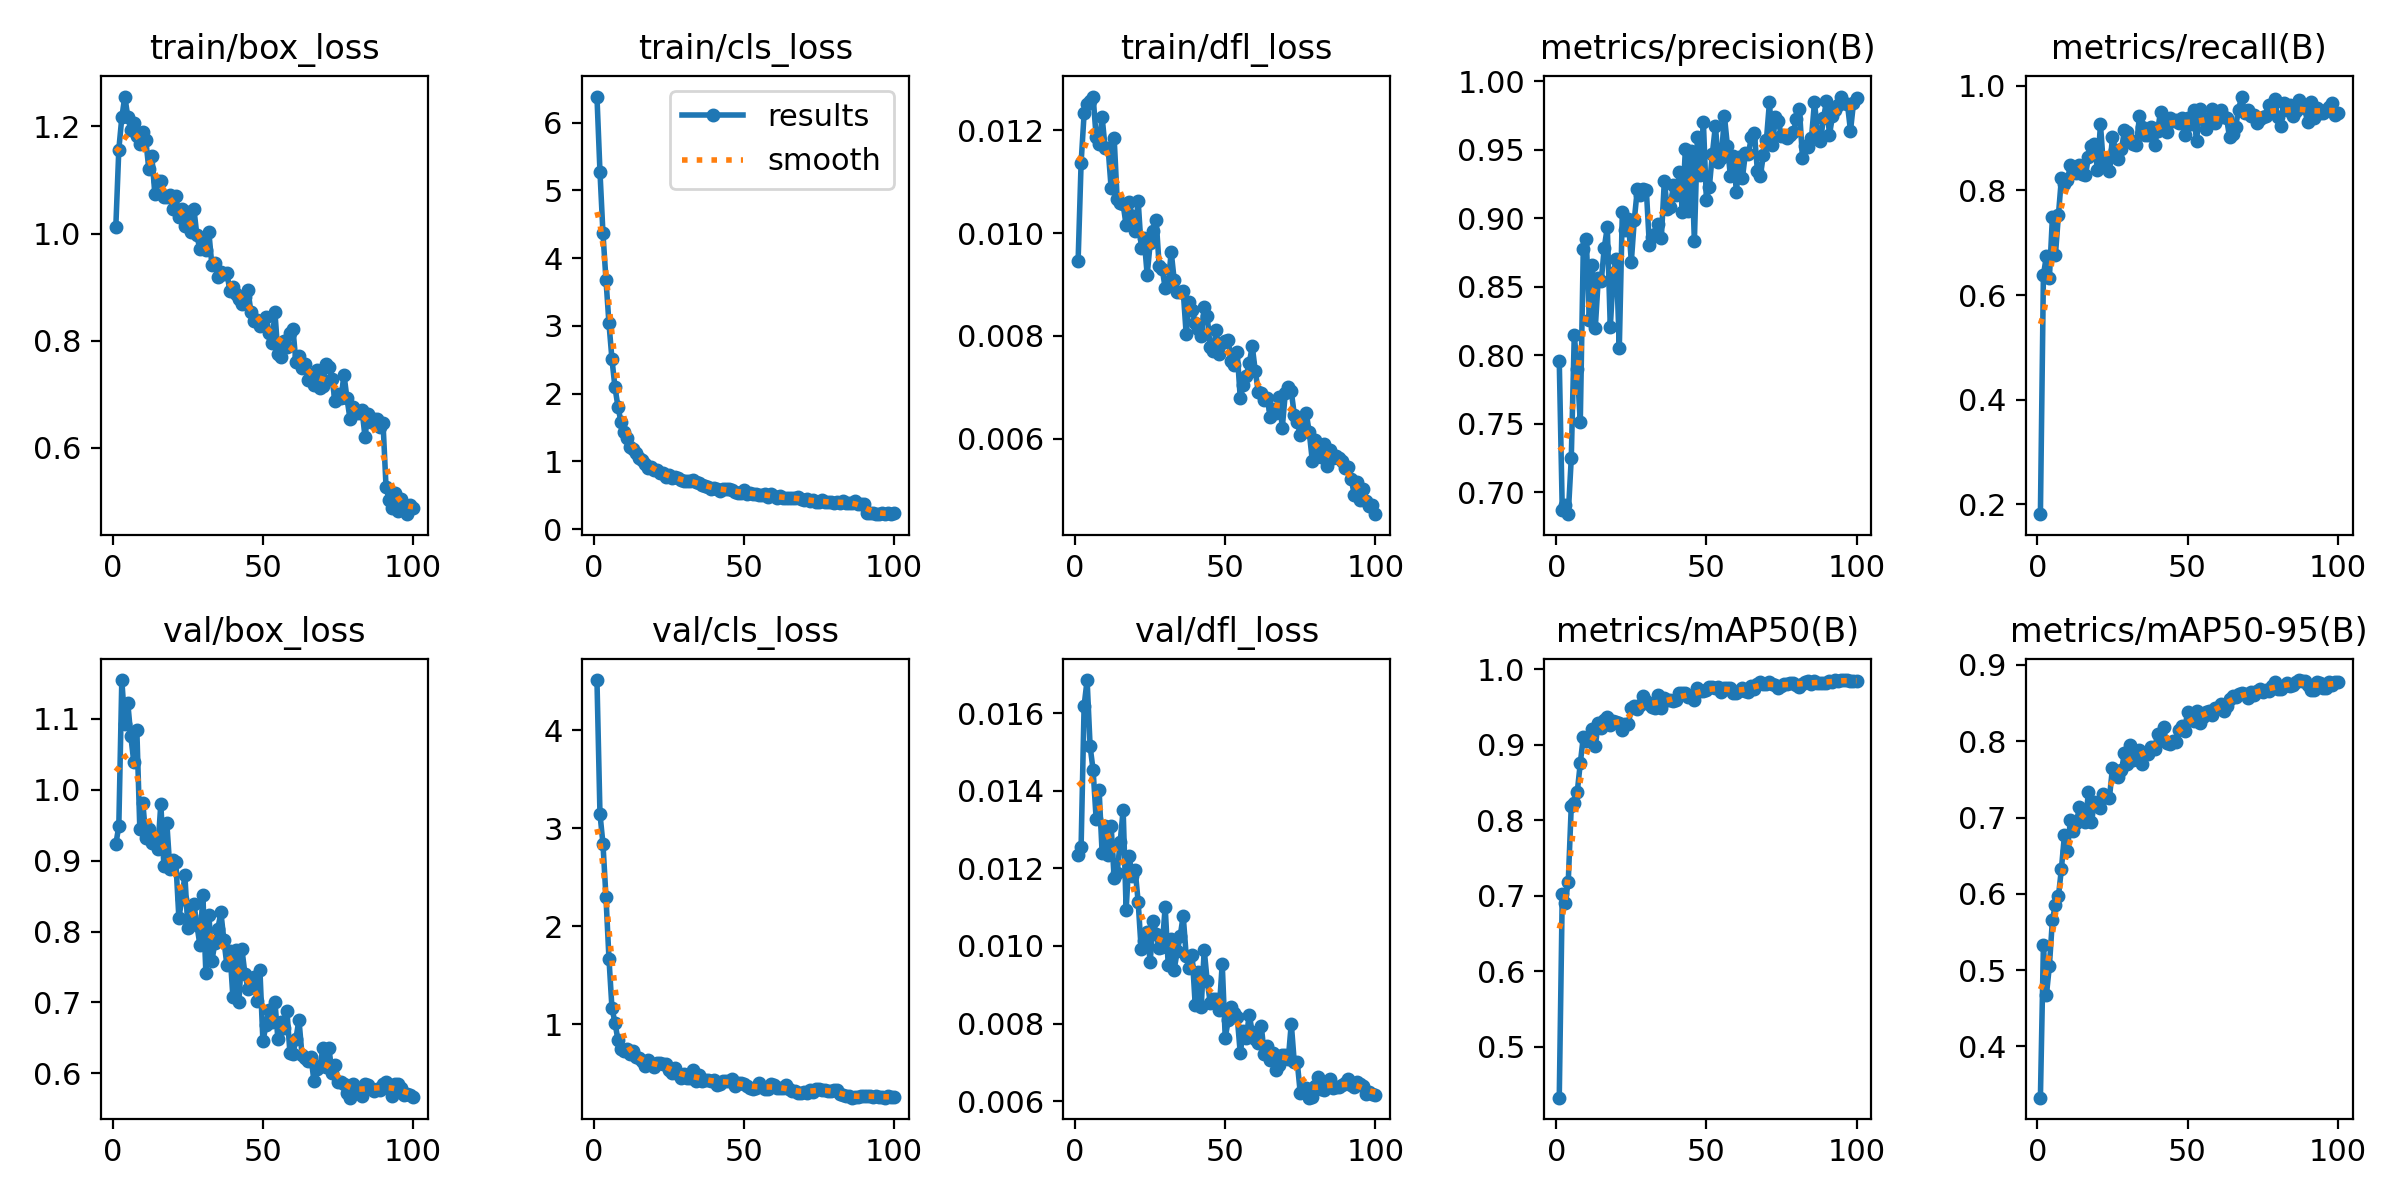
\includegraphics[width=0.96\textwidth]{training_results.png}
  \caption{YOLO26n完整100轮训练与验证曲线}
  \label{fig:training}
\end{figure}

\subsection{最佳验证指标与模型固化}

\begin{table}[H]
  \centering
  \caption{最佳权重的验证集指标}
  \begin{tabular}{lr}
    \toprule
    指标 & 数值 \\
    \midrule
    Precision & 0.96338 \\
    Recall & 0.97329 \\
    mAP@0.5 & 0.98185 \\
    mAP@0.5:0.95 & 0.88025 \\
    最佳轮次 & 87 \\
    \bottomrule
  \end{tabular}
\end{table}

最终权重复制到\path{models/pencil_tennis_yolo26n_best.pt}，并以模型卡记录训练参数、评价结果、部署环境、限制及SHA-256。验证指标只用于描述模型选择过程，不能代替独立测试和课程验收。

\section{独立测试集评估}

\subsection{总体及逐类结果}

模型确定后，由\path{src/evaluate_yolo26n_windows.py}在119张留出测试图片上执行评估。总体Precision为0.98877，Recall为0.90186；mAP50为0.97148，mAP50--95为0.87761。表\ref{tab:testmetrics}表明铅笔定位更稳定，网球Recall和高IoU指标相对较低，说明小目标或复杂背景下仍有漏检和定位误差。

\begin{table}[H]
  \centering
  \caption{独立测试集逐类指标}
  \label{tab:testmetrics}
  \begin{tabular}{lrrrrrr}
    \toprule
    类别 & 图片 & 目标 & P & R & mAP50 & mAP50--95 \\
    \midrule
    pencil & 60 & 80 & 1.0000 & 0.9466 & 0.9941 & 0.9542 \\
    tennis\_ball & 59 & 70 & 0.9775 & 0.8571 & 0.9489 & 0.8010 \\
    \midrule
    总体 & 119 & 150 & 0.9888 & 0.9019 & 0.9715 & 0.8776 \\
    \bottomrule
  \end{tabular}
\end{table}

\subsection{PR曲线与混淆矩阵}

图\ref{fig:pr}给出了独立测试的PR曲线。两类曲线均靠近左上区域，说明在较宽的置信度阈值范围内具有较好的Precision--Recall平衡。该图由Ultralytics标准评估流程生成，报告直接保留其原始彩色样式与数据。

\begin{figure}[H]
  \centering
  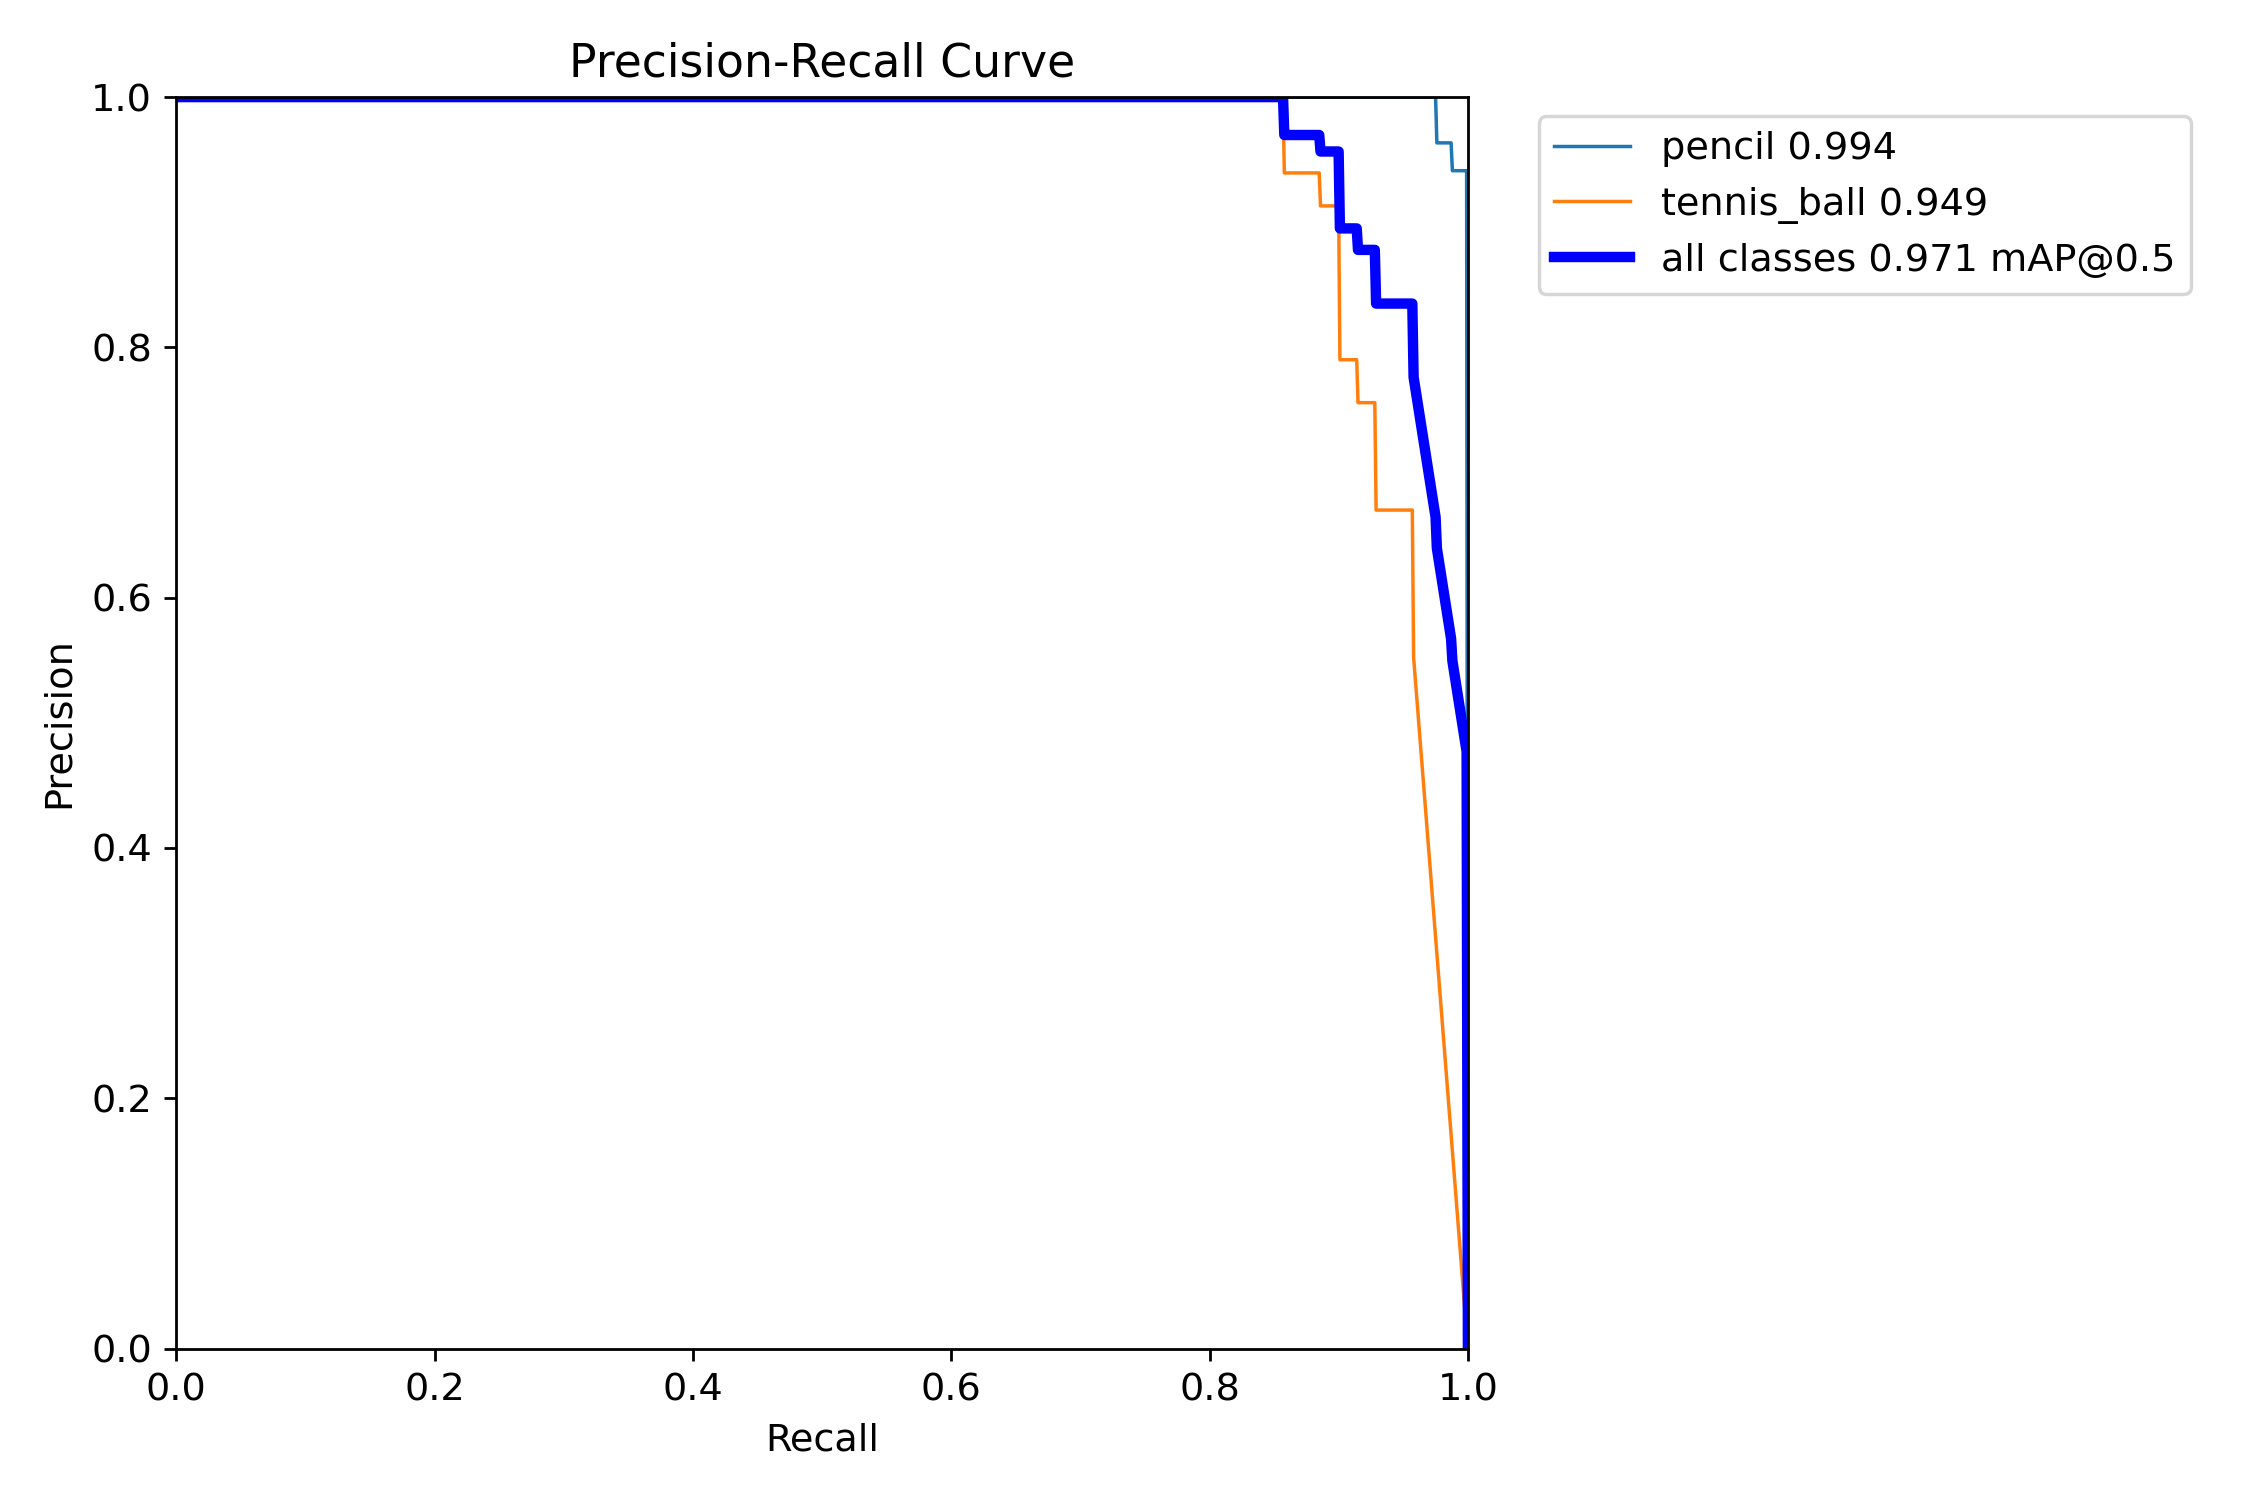
\includegraphics[width=0.82\textwidth]{test_pr_curve.png}
  \caption{独立测试集PR曲线}
  \label{fig:pr}
\end{figure}

图\ref{fig:confusion}为归一化混淆矩阵。铅笔正确分类比例约0.99，网球正确分类比例约0.89；主要问题表现为目标被归入背景，即漏检，而不是铅笔和网球相互混淆。该结论与网球Recall低于铅笔的逐类指标一致。

\begin{figure}[H]
  \centering
  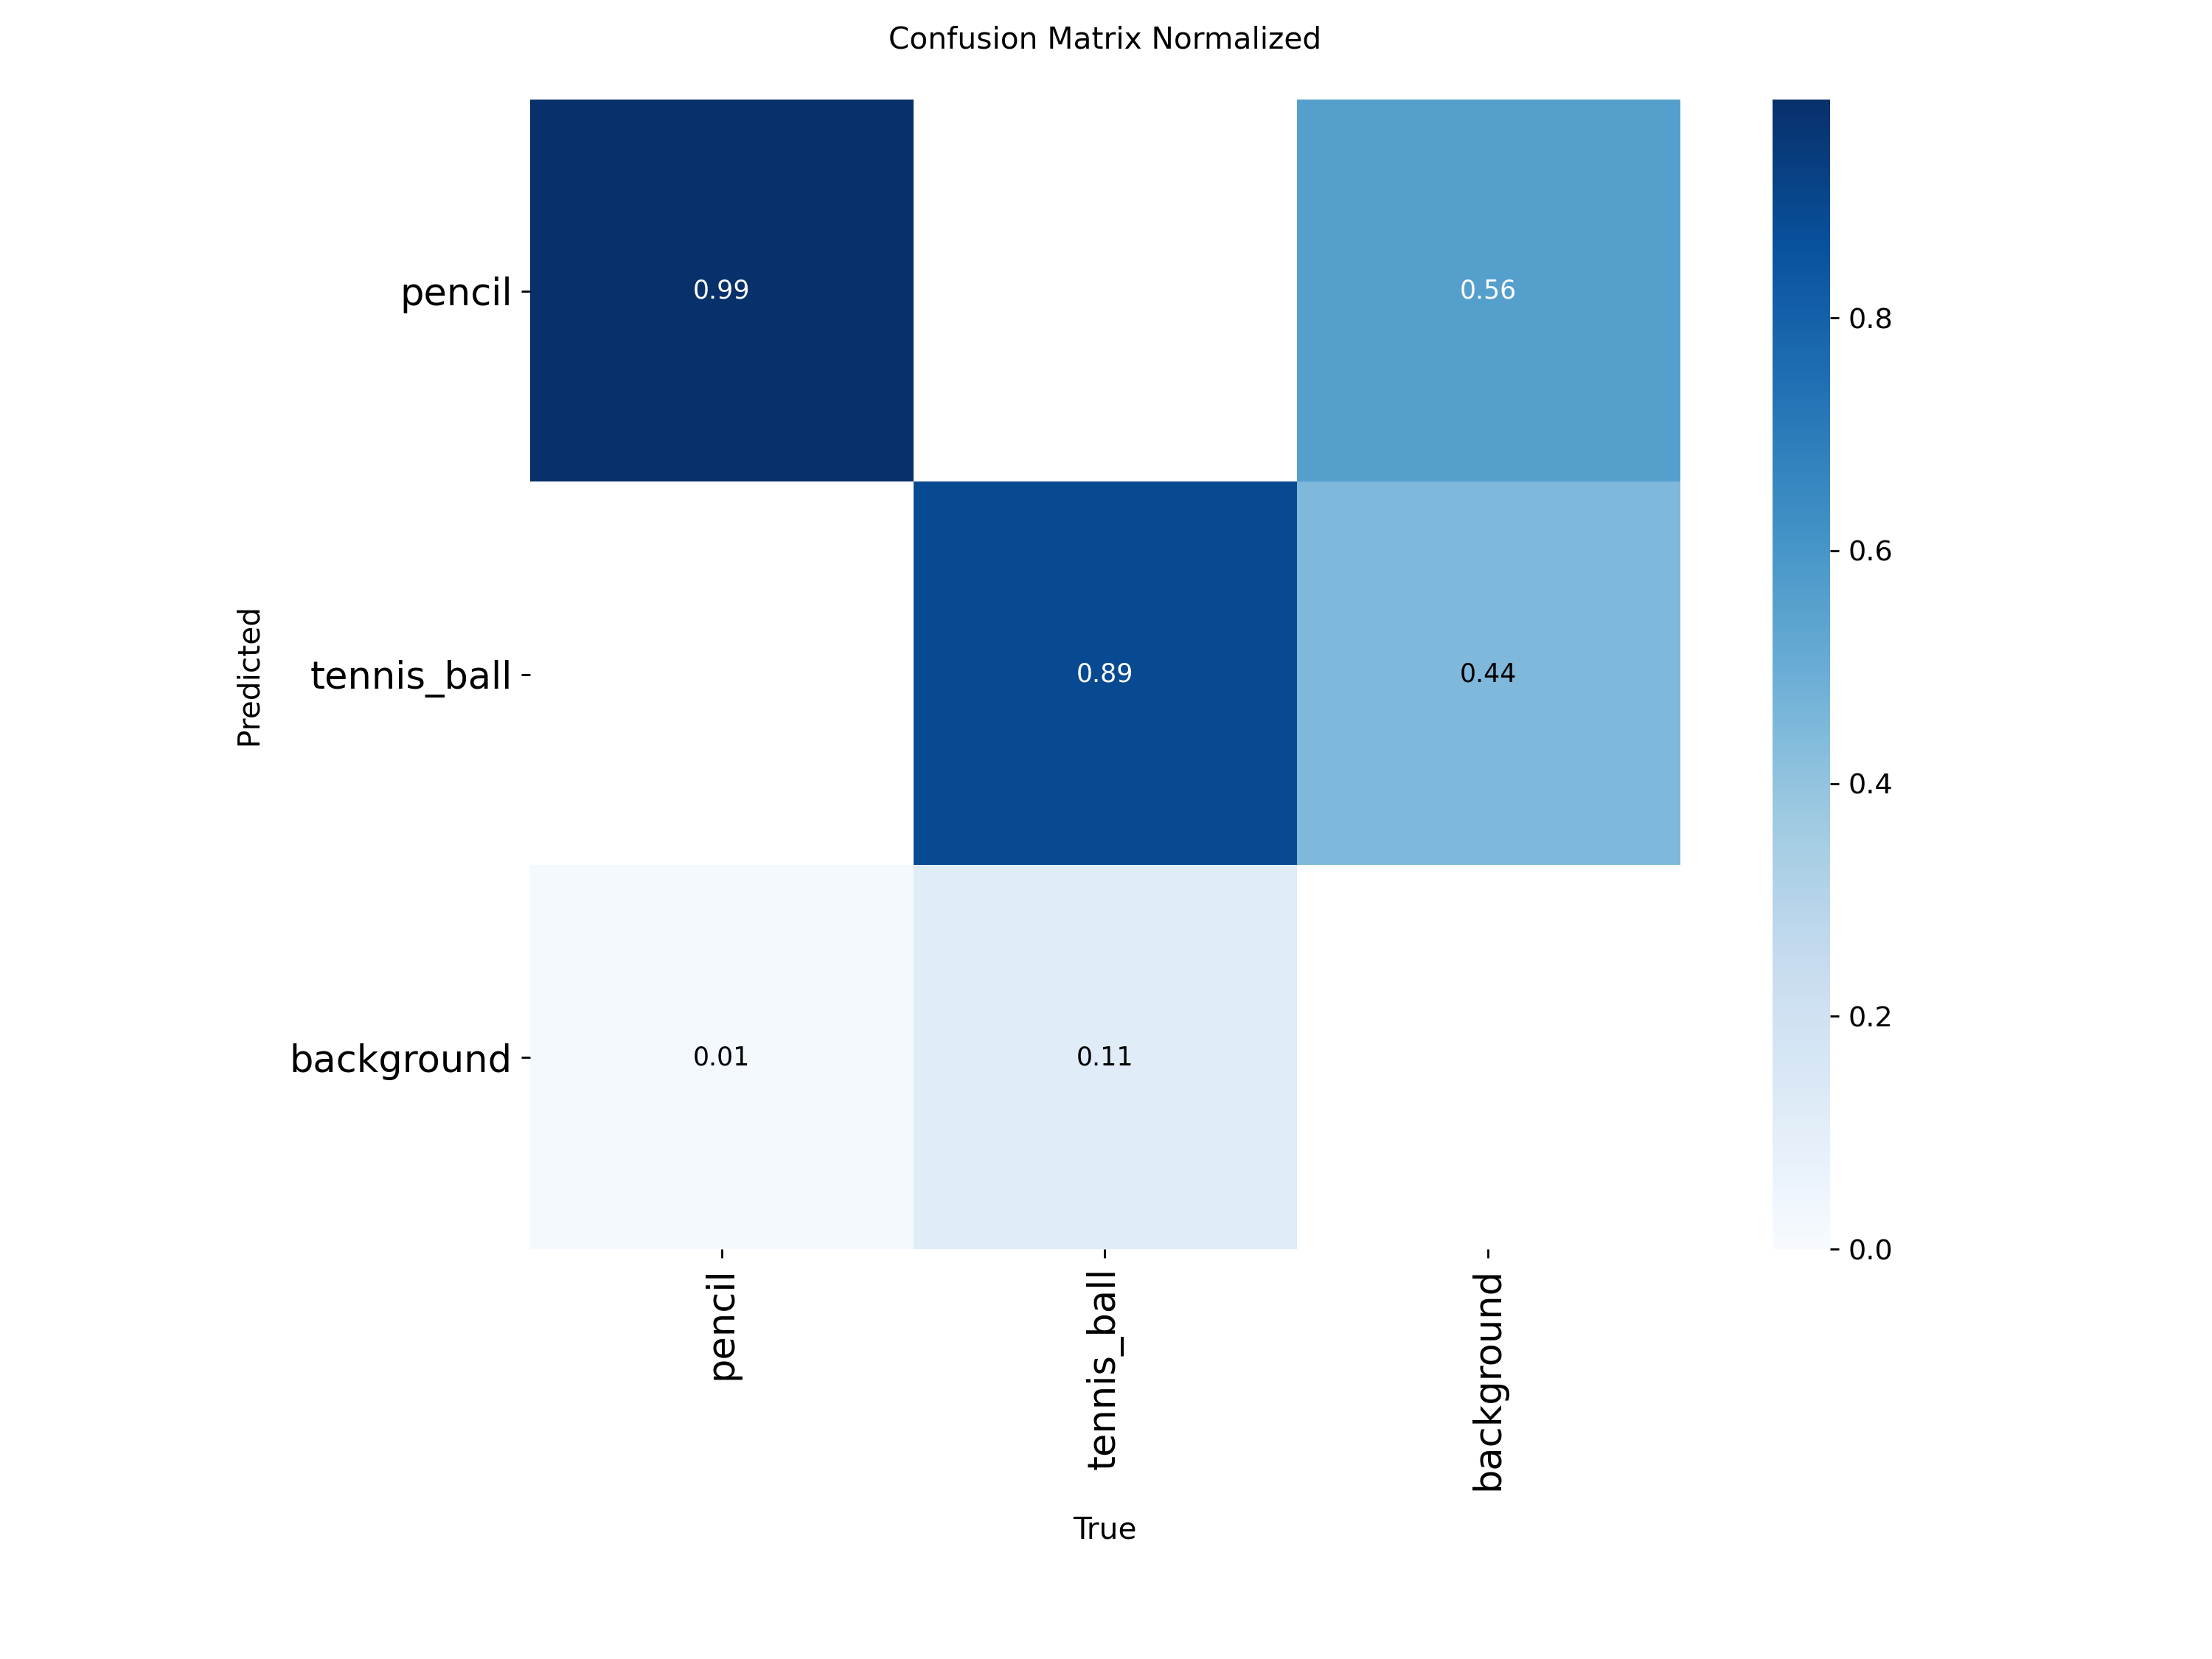
\includegraphics[width=0.78\textwidth]{test_confusion_matrix.png}
  \caption{独立测试集归一化混淆矩阵}
  \label{fig:confusion}
\end{figure}

\subsection{测试集检测样例}

图\ref{fig:penciltest}和图\ref{fig:tennistest}分别展示铅笔与网球预测样例。两张图片均来自119张测试集预测结果，不是人工绘制示意图。模型能够输出类别、置信度和边界框，满足可视化要求。

\begin{figure}[H]
  \centering
  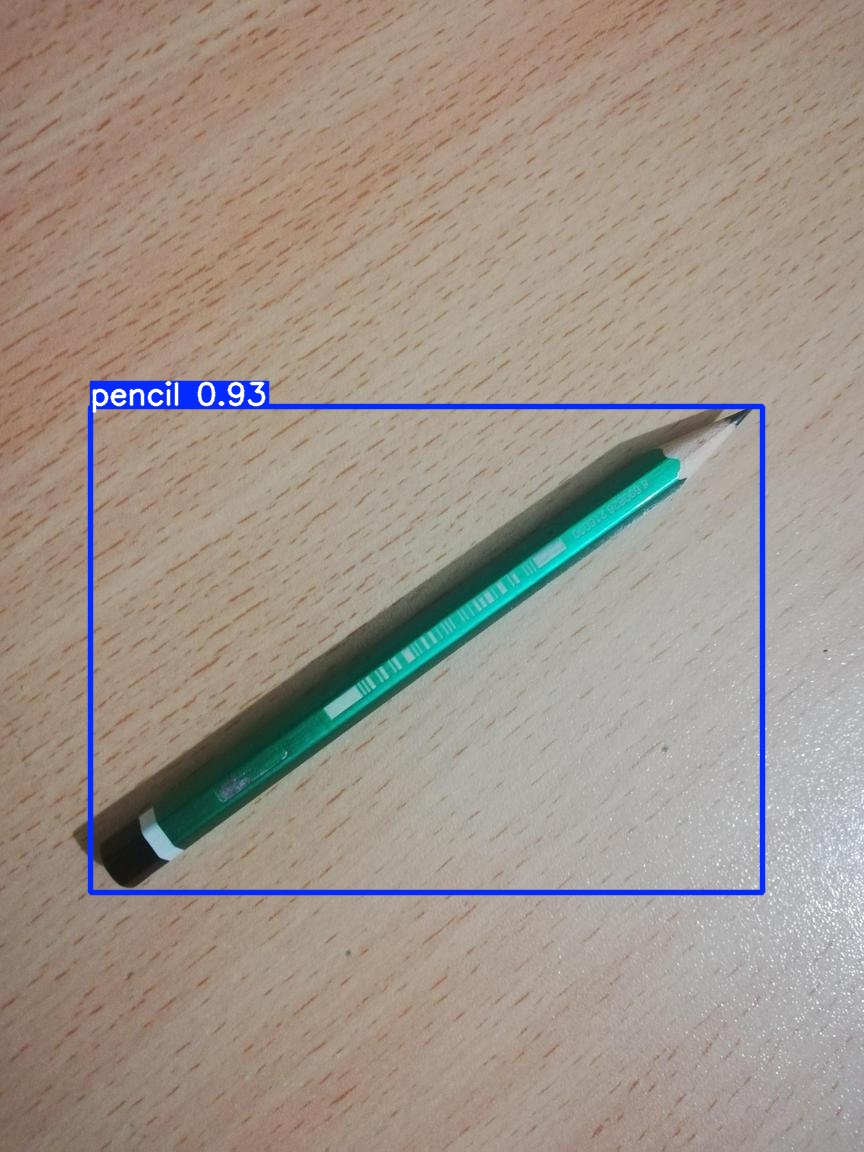
\includegraphics[width=0.48\textwidth]{detection_pencil.png}
  \caption{测试集铅笔检测样例}
  \label{fig:penciltest}
\end{figure}

\begin{figure}[H]
  \centering
  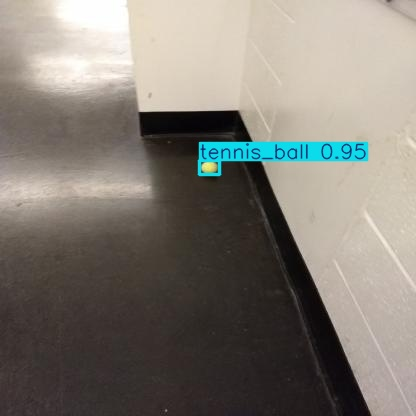
\includegraphics[width=0.40\textwidth]{detection_tennis.png}
  \caption{测试集网球检测样例}
  \label{fig:tennistest}
\end{figure}

\section{模型导出与Jetson部署}

\subsection{三种模型格式}

PyTorch权重用于复现与继续训练，ONNX用于跨框架交换，TensorRT Engine用于本次Jetson环境的高效推理。TensorRT提供面向NVIDIA GPU的推理运行时和性能优化能力\cite{tensorrt}。Engine与JetPack、TensorRT、CUDA、GPU架构和构建配置相关，不能假设在其他设备上直接兼容；环境变化时应从PT或ONNX重新导出。

\begin{table}[H]
  \centering
  \caption{最终模型文件与完整性记录}
  \begin{tabularx}{\textwidth}{Y r Y}
    \toprule
    文件 & 大小/byte & SHA-256（缩写） \\
    \midrule
    \path{pencil_tennis_yolo26n_best.pt} & 5,415,023 & DA747F4ED471BE2A\ldots A4063D \\
    \path{pencil_tennis_yolo26n_best.onnx} & 9,761,287 & 4616C124B10E4B2C\ldots C2401 \\
    \path{pencil_tennis_yolo26n_best.engine} & 7,863,922 & BBFFFC6D678DDF86\ldots DC0E3 \\
    \bottomrule
  \end{tabularx}
\end{table}

\subsection{板端环境与实时结果}

部署设备为Jetson Orin（aarch64），Jetson Linux为R36.4.3，CUDA 12.6可用，TensorRT 10.3.0，PyTorch 2.10.0，ROS 2使用Humble版本\cite{ros2humble}。USB摄像头通过V4L2 MJPG方式采集，分辨率为$640\times480$，缓冲区设为1以降低累积延迟。

图\ref{fig:jetson}截取自最终提交视频第8秒。画面中同时存在铅笔和网球，检测框、类别、置信度和实时FPS均清晰显示；该帧FPS为16.7。最终视频时长29.76秒，采用H.264/AAC编码，保存于\path{results/jetson/2026-08-30/jetson_demo.mp4}。

\begin{figure}[H]
  \centering
  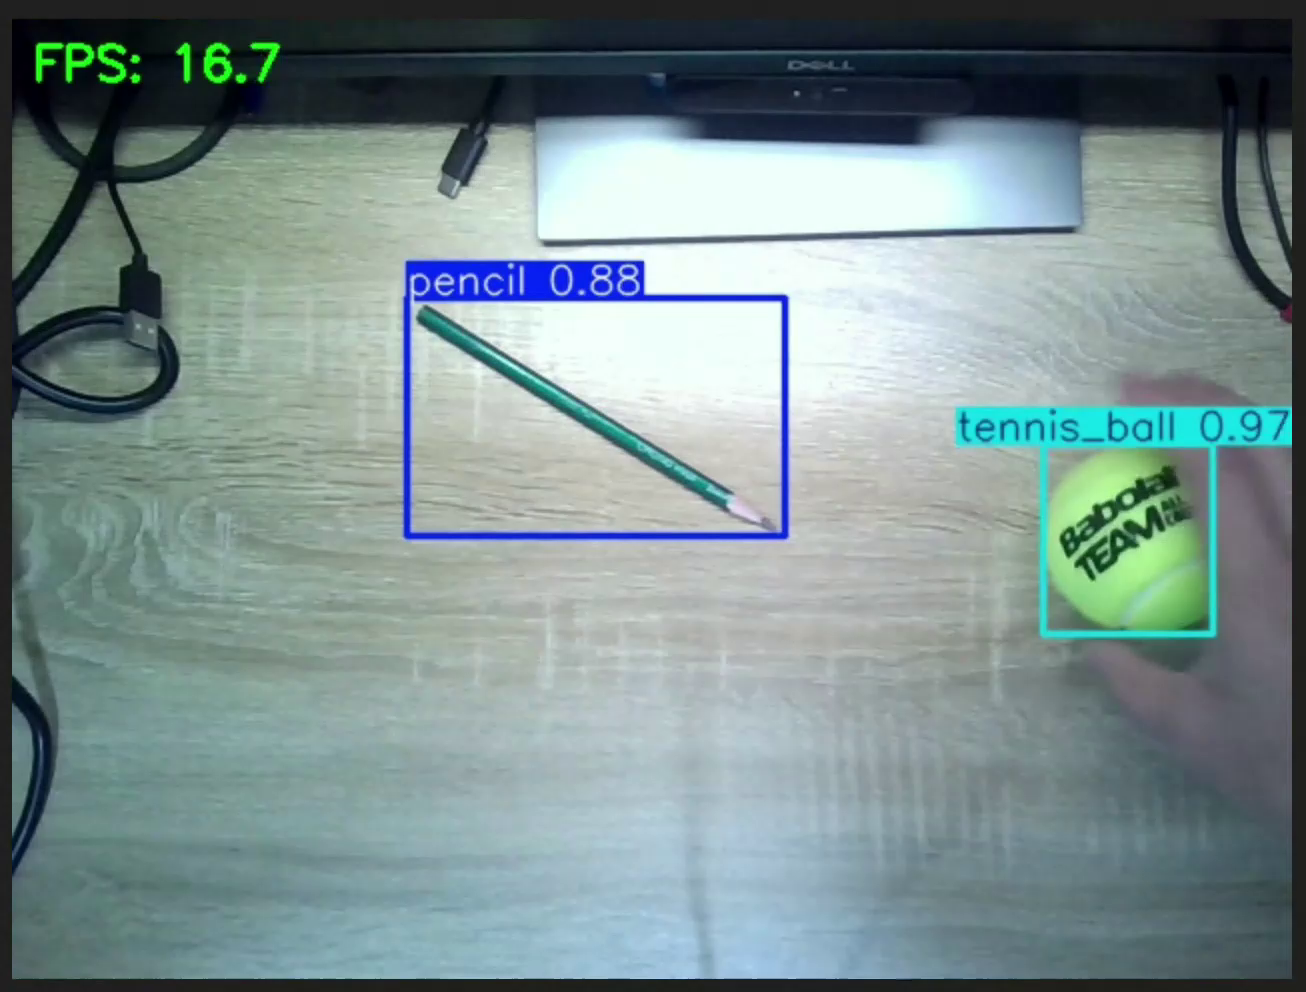
\includegraphics[width=0.92\textwidth]{jetson_realtime.png}
  \caption{Jetson最终视频第8秒实时检测画面}
  \label{fig:jetson}
\end{figure}

\begin{table}[H]
  \centering
  \caption{Jetson实时速度记录}
  \begin{tabular}{lrrrr}
    \toprule
    统计对象 & 样本数 & 最低/FPS & 平均/FPS & 最高/FPS \\
    \midrule
    \path{/detection/image}话题速率 & 5 & 13.369 & 13.795 & 14.092 \\
    \path{/detection/fps}发布数据 & 46 & 15.421 & 16.657 & 17.971 \\
    \bottomrule
  \end{tabular}
\end{table}

图像话题速率更接近包含采集、推理、绘制和发布的实际输出吞吐量。FPS话题记录的是节点按单帧处理耗时计算并发布的检测速度。两个口径的最低记录都大于5 FPS，因此实时性能验收通过。

\section{ROS 2节点与话题设计}

\subsection{检测节点}

ROS 2包保存在仓库的\path{ros2_ws}目录。检测节点\path{detector_node.py}完成摄像头采集、YOLO推理、结果解析、图像绘制与三类消息发布。节点名为\path{/pencil_tennis_detector}，参数包括模型路径、摄像头编号、置信度阈值、输入尺寸、CUDA设备和定时器周期。ROS 2的节点和话题机制使检测器与显示、记录或机器人控制模块解耦。

\begin{figure}[H]
  \centering
  \begin{tikzpicture}[
    node distance=6mm,
    box/.style={draw=black,minimum height=9mm,text width=3.0cm,align=center,font=\small},
    topic/.style={draw=black,rounded corners=1pt,minimum height=8mm,text width=3.6cm,align=center,font=\small},
    arrow/.style={-Latex,thick}
  ]
    \node[box] (camera) {USB摄像头\\V4L2 MJPG};
    \node[box,right=of camera] (node) {检测节点\\YOLO + OpenCV};
    \node[topic,right=of node,yshift=12mm] (image) {\path{/detection/image}\\sensor\_msgs/Image};
    \node[topic,right=of node] (results) {\path{/detection/results}\\std\_msgs/String};
    \node[topic,right=of node,yshift=-12mm] (fps) {\path{/detection/fps}\\std\_msgs/Float32};
    \draw[arrow] (camera) -- (node);
    \draw[arrow] (node) -- (image);
    \draw[arrow] (node) -- (results);
    \draw[arrow] (node) -- (fps);
  \end{tikzpicture}
  \caption{ROS 2检测节点与话题关系}
  \label{fig:ros}
\end{figure}

\subsection{消息内容}

\begin{table}[H]
  \centering
  \caption{ROS 2话题设计}
  \begin{tabularx}{\textwidth}{Y Y Y}
    \toprule
    话题 & 消息类型 & 内容与用途 \\
    \midrule
    \path{/detection/image} & \path{sensor_msgs/Image} & 带检测框、类别、置信度和FPS的图像 \\
    \path{/detection/results} & \path{std_msgs/String} & 每帧JSON结果，含类别、置信度和边界框 \\
    \path{/detection/fps} & \path{std_msgs/Float32} & 单帧处理速度，供监控与验收记录 \\
    \bottomrule
  \end{tabularx}
\end{table}

结构化检测结果包含时间戳、帧号、图像尺寸和检测数组。真实部署记录中的一个网球样例置信度为0.958984375，边界框采用像素坐标$(x_1,y_1,x_2,y_2)$。这种JSON形式便于调试，也方便后续机器人节点订阅；若进入规模化系统，可进一步定义专用ROS 2消息，避免字符串解析开销。

\begin{lstlisting}[language={},caption={检测结果JSON结构示例}]
{
  "frame_id": 6710,
  "image_width": 640,
  "image_height": 480,
  "detections": [{
    "class_id": 1,
    "class_name": "tennis_ball",
    "confidence": 0.958984375,
    "bbox": {"x1":145.625,"y1":168.0,
             "x2":313.5,"y2":332.0}
  }]
}
\end{lstlisting}

\section{最终40项验收与错误分析}

\subsection{测试方法}

板端共保留两次离线验收。第一次10张铅笔加10张网球仅作为初步记录；第二次才是最终验收。最终测试固定随机种子20260830，只从\path{dataset/images/test}抽取互不重复的40张图片，验证集未参与选样。前20项为铅笔、后20项为网球，每张图恰含一个真实标注目标。模型使用正式TensorRT Engine，置信度阈值为0.25；最高置信度检测决定预测类别，空检测记为错误。测试脚本、CSV、JSON、日志及40张带标注结果图均保存在\path{results/jetson/2026-08-30/acceptance/attempt_02}。

\subsection{结果统计}

\begin{table}[H]
  \centering
  \caption{Jetson第二次最终验收结果}
  \begin{tabular}{lrrrr}
    \toprule
    类别 & 测试数 & 正确数 & 错误数 & 正确率 \\
    \midrule
    pencil & 20 & 19 & 1 & 95.0\% \\
    tennis\_ball & 20 & 20 & 0 & 100.0\% \\
    \midrule
    总计 & 40 & 39 & 1 & 97.5\% \\
    \bottomrule
  \end{tabular}
\end{table}

40项总正确率为
\begin{equation}
  \mathrm{Accuracy}=\frac{39}{40}\times100\%=97.5\%,
\end{equation}
比80\%验收线高17.5个百分点。离线TensorRT模型平均速度为31.7906 FPS，最低为30.1659 FPS。该速度由Ultralytics预处理、推理和后处理时间计算，不包含摄像头采集和ROS 2发布，故只作为模型端性能补充，不替代上一章的摄像头实时速度。

图\ref{fig:acceptcorrect}为最终验收中的网球正确案例。文本记录了测试序号、真实类别、预测类别、置信度、结果与离线模型FPS，使单项结果可追溯。

\begin{figure}[H]
  \centering
  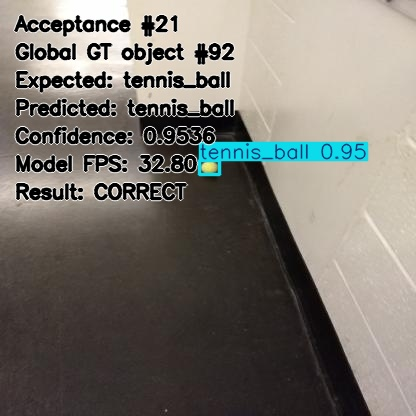
\includegraphics[width=0.72\textwidth]{acceptance_correct.png}
  \caption{最终40项验收中的网球正确案例}
  \label{fig:acceptcorrect}
\end{figure}

\subsection{唯一错误案例}

唯一错误是\path{pencil_red4.jpg}漏检，如图\ref{fig:accepterror}所示。模型没有输出高于0.25阈值的检测框，因此预测类别为空、置信度记为0。该样本未被删除、替换或重新抽样，确保验收记录真实完整。

\begin{figure}[H]
  \centering
  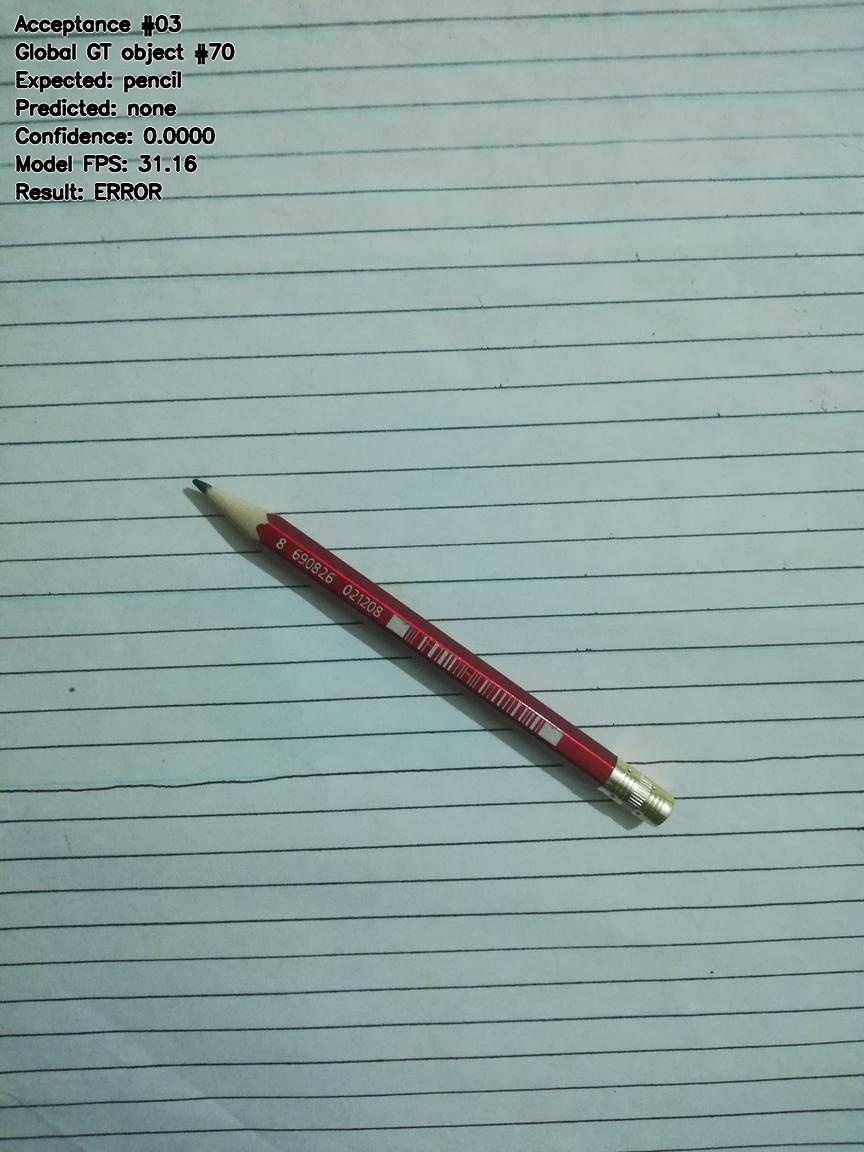
\includegraphics[width=0.78\textwidth]{acceptance_error.png}
  \caption{最终验收唯一错误：红色铅笔漏检}
  \label{fig:accepterror}
\end{figure}

从图像观察，铅笔目标细长、与横线背景存在结构干扰，且目标在画面中占比较小。结合独立测试混淆矩阵，当前主要风险是目标被归为背景，而不是两类互相混淆。改进方向包括补充低对比度细长目标、混合桌面背景和两类同时出现的真实图片；在不显著增加误检的前提下重新标定置信度阈值；以及比较更高分辨率输入或小目标检测头。由于当前结果已经超过课程阈值，本报告未用错误样本反向调整模型后重新测试，以避免测试集泄漏。

\section{GitHub过程管理与材料完整性}

\subsection{公开仓库与连续提交}

项目仓库为Public，地址如下：

\noindent\githuburl

报告、代码、数据、模型、测试图表、Jetson证据、最终视频和运行说明均按目录组织。图\ref{fig:githubrepo}为2026年8月30日抓取的真实公开仓库页面，可见主分支、项目目录和当时30次提交记录。

\begin{figure}[H]
  \centering
  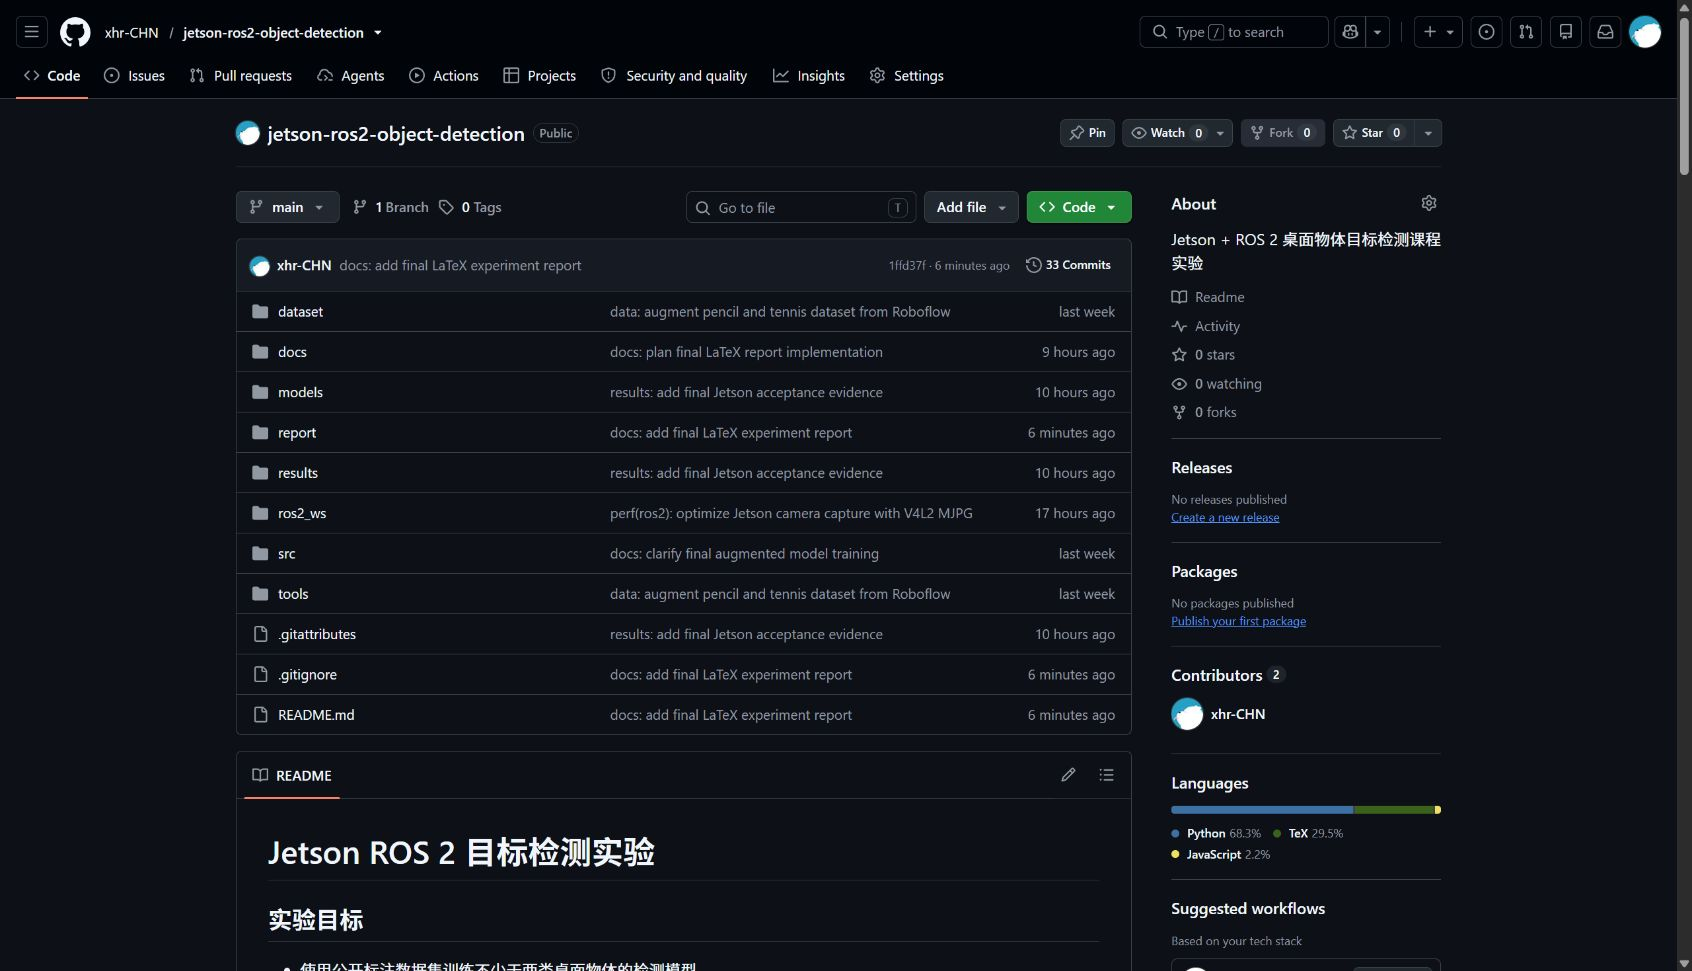
\includegraphics[width=0.98\textwidth]{github_repository.png}
  \caption{GitHub公开仓库页面截图}
  \label{fig:githubrepo}
\end{figure}

项目没有采用单次全量提交，而是按数据、训练、推理、ROS 2、模型导出、Jetson证据、视频和验收结果逐步提交。图\ref{fig:githubcommits}展示真实提交历史；报告设计、实现与最终PDF在该截图之后继续形成独立提交，因此截图主要证明实验主体的连续过程记录。

\begin{figure}[H]
  \centering
  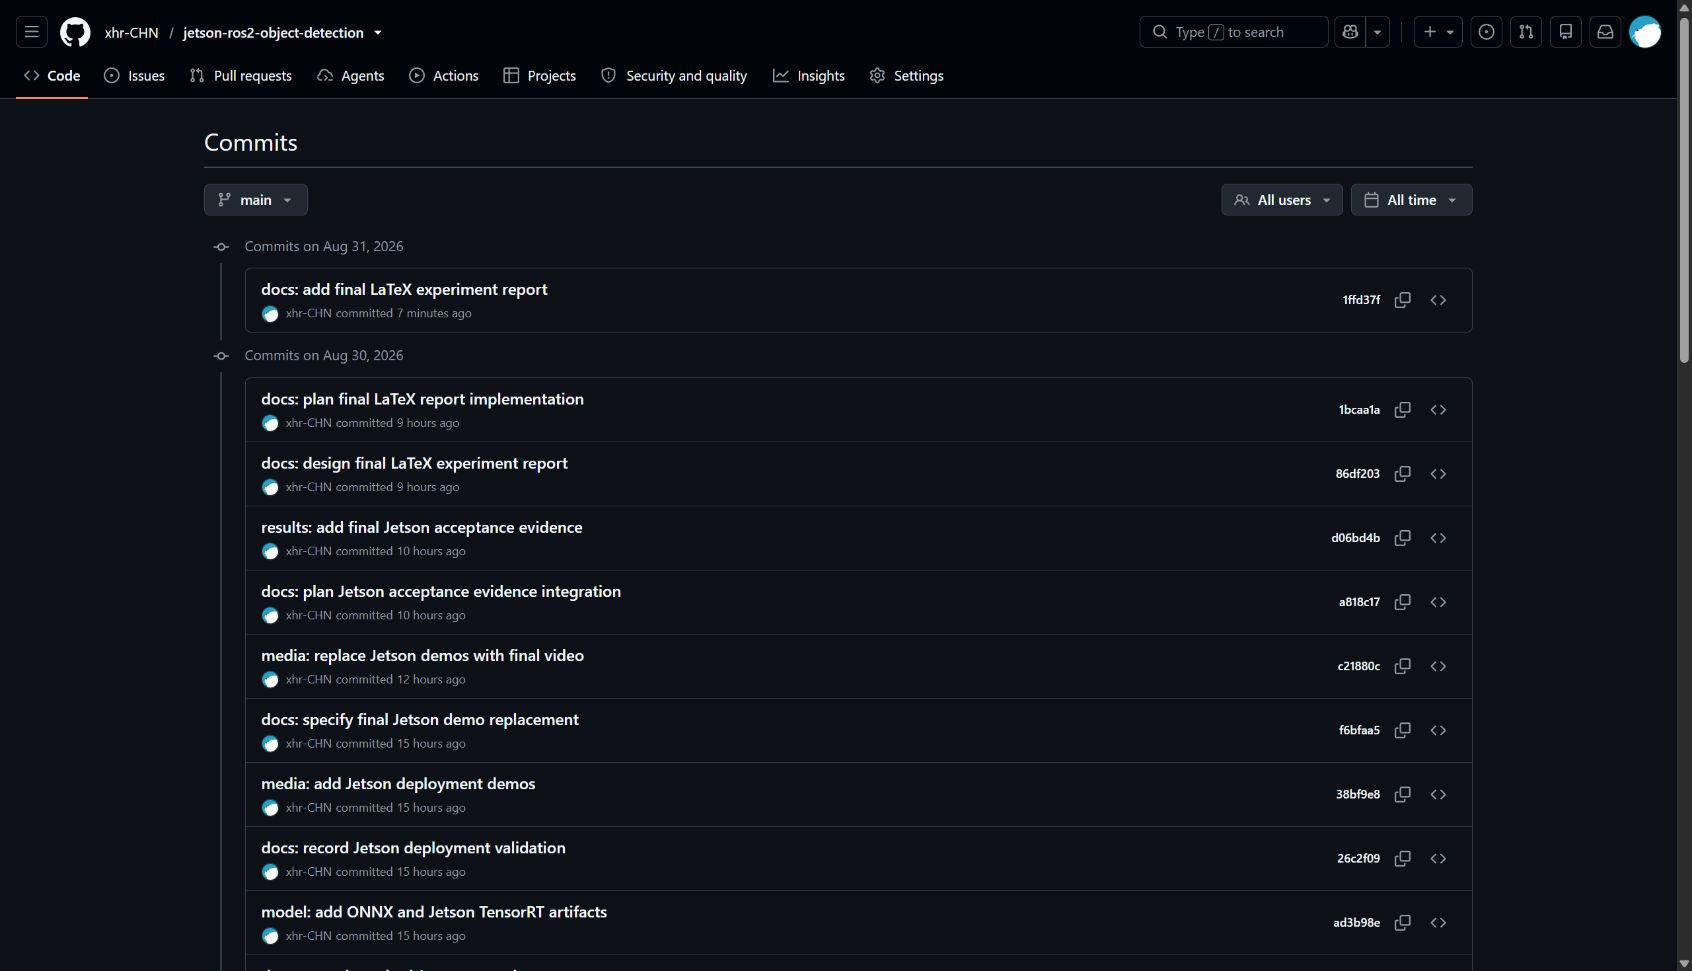
\includegraphics[width=0.98\textwidth]{github_commits.png}
  \caption{GitHub主分支连续提交记录截图}
  \label{fig:githubcommits}
\end{figure}

\begin{longtable}{p{1.7cm}p{3.5cm}p{8.7cm}}
  \caption{代表性Git提交记录}\label{tab:commits}\\
  \toprule
  提交 & 类型 & 内容 \\
  \midrule
  \endfirsthead
  \toprule
  提交 & 类型 & 内容 \\
  \midrule
  \endhead
  4ee5a04 & data & 合并Roboflow铅笔和网球补充数据 \\
  2e385b3 & train & 增加增强YOLO26n正式训练模式 \\
  9e616f5 & feat & 增加增强模型摄像头实时检测 \\
  77a9956 & model & 固化完整100轮训练的最终最佳权重 \\
  85923cb & test & 对最终增强模型执行独立测试 \\
  2e907f8 & docs & 澄清最终模型来自完整100轮训练 \\
  2e15f0d & perf(ros2) & 使用V4L2 MJPG优化Jetson摄像头采集 \\
  ad3b98e & model & 加入ONNX和Jetson TensorRT产物 \\
  26c2f09 & docs & 记录Jetson系统、话题和速度验证 \\
  c21880c & media & 用最终Jetson演示视频替换早期视频 \\
  a818c17 & docs & 制定最终验收证据集成计划 \\
  d06bd4b & results & 提交Jetson第二次40项最终验收证据 \\
  \bottomrule
\end{longtable}

\subsection{最终提交材料}

\begin{table}[H]
  \centering
  \caption{最终GitHub提交材料清单}
  \begin{tabularx}{\textwidth}{Y Y}
    \toprule
    目录/文件 & 内容 \\
    \midrule
    \path{dataset/} & 895张图片、YOLO标签、配置、来源与整理统计 \\
    \path{models/} & PT、ONNX、TensorRT Engine及模型卡 \\
    \path{src/} & Windows训练、评估和摄像头检测程序 \\
    \path{ros2_ws/} & ROS 2检测节点、验收记录节点、启动文件和测试 \\
    \path{results/training/} & 100轮训练参数、CSV、曲线与混淆矩阵 \\
    \path{results/test/} & 119张测试预测、指标、PR曲线和混淆矩阵 \\
    \path{results/jetson/} & 板端环境、速度、40项验收、错误案例和最终视频 \\
    \path{README.md} & Windows、Ubuntu/Jetson与ROS 2运行说明 \\
    \path{report/} & LaTeX源码、参考资料、真实证据图和最终PDF \\
    \bottomrule
  \end{tabularx}
\end{table}

Kaggle铅笔数据的许可证仍需谨慎处理，这是材料完整性之外的合规限制。仓库保留了来源与风险说明，便于教师核查，也为后续替换为明确许可的数据集留下依据。

\section{结论与改进方向}

本实验完成了从数据到边缘部署的完整目标检测流程。最终数据集包含895张图片和1048个目标；YOLO26n完成100轮训练，最佳权重来自第87轮；独立测试集mAP@0.5达到0.97148，mAP@0.5:0.95达到0.87761；Jetson摄像头图像话题平均速率13.795 FPS；ROS 2成功发布检测图像、结构化结果和FPS；最终第二次40项验收正确39项，总正确率97.5\%。这些结果均由CSV、JSON、曲线、混淆矩阵、图片、日志、视频和Git提交记录支撑。

实验中最重要的工程认识有三点。第一，验证集、独立测试集和课程验收具有不同用途，不能用同一个百分比替代所有结论。第二，TensorRT Engine具有环境相关性，模型哈希、软件版本和部署平台必须一起记录。第三，只有保留错误案例和完整提交历史，结果才具有可追溯性；本实验保留了唯一漏检样本，并未为了提高统计结果而删除或重抽。

后续改进可从三方面开展：一是采集更多铅笔和网球同时出现、低照度、遮挡和复杂桌面的真实数据；二是建立现场摄像头逐个摆放实物的人工验收表，与当前固定测试集验收相互补充；三是将JSON字符串消息升级为自定义ROS 2检测消息，并为下游抓取或跟踪模块加入时间同步与坐标转换。若更换JetPack或Jetson型号，应重新导出TensorRT Engine并重复速度和正确率验收。

\clearpage
\begingroup\sloppy
\begin{thebibliography}{99}
\addcontentsline{toc}{section}{参考文献}

\bibitem{yolo26paper}
Jocher G, Qiu J, Liu M, et al. Ultralytics YOLO26: Unified Real-Time End-to-End Vision Models[EB/OL]. arXiv:2606.03748, 2026. \url{https://arxiv.org/abs/2606.03748}.

\bibitem{yolo26docs}
Ultralytics. Ultralytics YOLO26 Documentation[EB/OL]. 2026[2026-08-30]. \url{https://docs.ultralytics.com/models/yolo26/}.

\bibitem{ros2humble}
Open Robotics. ROS 2 Humble Documentation[EB/OL]. [2026-08-30]. \url{https://docs.ros.org/en/humble/}.

\bibitem{tensorrt}
NVIDIA Corporation. NVIDIA TensorRT Documentation[EB/OL]. [2026-08-30]. \url{https://docs.nvidia.com/deeplearning/tensorrt/latest/}.

\bibitem{mendeley}
Jagtiani K. Object Detection--Tennis Ball, Version 2[DS/OL]. Mendeley Data, 2021. DOI:10.17632/ppr8rdw98w.2.

\bibitem{kagglepencil}
Saglam F. Pencil Dataset[DS/OL]. Kaggle, 2023[2026-08-24]. \url{https://www.kaggle.com/datasets/greysky/pencil-dataset}.

\bibitem{roboflowpencil}
Roboflow Universe. Pencil Dataset, Version 2[DS/OL]. [2026-08-24]. \url{https://universe.roboflow.com/workspace1-1gbmx/pencil-tvhes/dataset/2}.

\bibitem{roboflowtennis}
Roboflow Universe. Tennis Ball Dataset, Version 1[DS/OL]. [2026-08-24]. \url{https://universe.roboflow.com/tennis-3ll0a/tennis-ball-icifx/dataset/1}.

\end{thebibliography}
\endgroup

\end{document}
